\problemname{Multationer}
\noindent

On the as yet undiscovered exoplanet PO-2019, the inhabitants' genetic material consists of a string
where each letter is either A, B, or C. The evolution of life has progressed a little faster
there than on Earth (for example, everyone can solve programming problems from birth).
The reason is believed to be that instead of ordinary mutations, ``multations'' occur,
which change {\em all} occurrences of a certain letter simultaneously.
The letter is replaced by a string that can contain 1, 2, or 3 letters (see the figure below).
This means that the length of the genetic material can increase rather quickly.

Write a program that, given two strings $S$ and $T$,
prints the shortest sequence of multations that changes $S$ to $T$.
There will always be a solution with at most $3$ multations.

\section*{Input}
The first line contains the string $S$. The second line contains the string $T$.
Neither string contains more than $10$ letters and each
letter is either A, B, or C.

\section*{Output}
The program should print one line for each multation, in the order they occur.
Each line should contain two strings: the letter that is changed, and the string it is changed to.

If there are multiple optimal sequences, you may print any of them.

\noindent
\begin{tabular}{| l | l | p{12cm} |}
  \hline
  \textbf{Group} & \textbf{Points} & \textbf{Constraints} \\ \hline
  $1$    & $20$       & $S$ and $T$ have the same length. \\ \hline
  $2$    & $40$       & There is an optimal sequence that consists only of the same multation, but possibly repeated multiple times. \\ \hline
  $3$    & $40$       & No additional constraints. \\ \hline
\end{tabular}


\begin{figure}[!h]
  \centering
      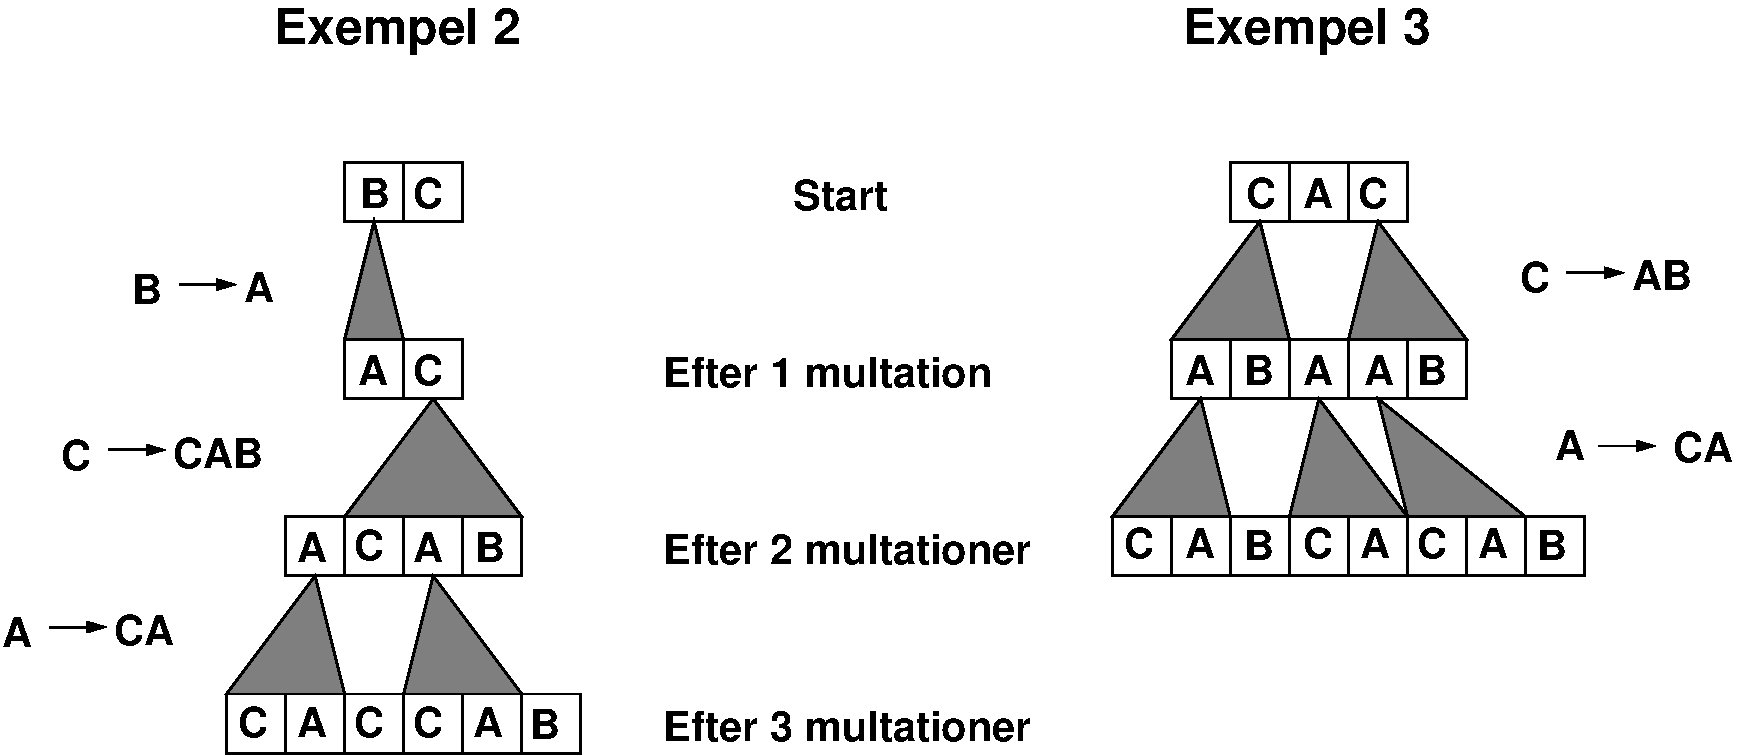
\includegraphics[width=0.9\textwidth]{multationer1.pdf}
\end{figure}
